% =====================================================================
%  Wuhan (Yb) - Shanghai (Sr) optical-clock comparison:
%  tidal gravitational-redshift detection and fixed-coefficient
%  tidal corrections.
%
%  Submission draft (deliverable A).
%  Every numeric claim carries a "% src:" comment pointing at the
%  repository artifact it was read from.  Two numbers that remain
%  provisional (author list; the experiment-side per-segment counts,
%  which differ from this work's endpoint-trimmed counts) are marked
%  in place.
%
%  Compile:  pdflatex main.tex && bibtex main && pdflatex main.tex && pdflatex main.tex
% =====================================================================
\documentclass[11pt,a4paper]{article}

\usepackage[T1]{fontenc}
\usepackage[utf8]{inputenc}
\usepackage{amsmath}
\usepackage{amssymb}
\usepackage{graphicx}
\usepackage{booktabs}
\usepackage{geometry}
\usepackage[hidelinks]{hyperref}

% siunitx is optional: this TeX Live install does not ship it.
% Define plain fallbacks first, then let siunitx override them if present.
\newcommand{\SI}[2]{#1\,#2}
\newcommand{\num}[1]{#1}
\IfFileExists{siunitx.sty}{%
  \usepackage{siunitx}%
  \sisetup{detect-all,separate-uncertainty=true}%
}{}

\geometry{margin=2.5cm}

\newcommand{\Rdur}{R_{\mathrm{duration}}}
\newcommand{\Rwls}{R_{\mathrm{wls}}}
\newcommand{\dff}{\Delta f/f}
\newcommand{\dW}{\Delta W}
\newcommand{\Ffifteen}{F_{1550}}
\newcommand{\e}[1]{\times 10^{#1}}

\title{An inter-city optical clock network for precision metrology
and relativistic geodesy}

\author{%
  Haifeng Jiang%
  % NOTE: author list and affiliations are provisional.
  % Co-authors and institutional affiliations to be supplied by the
  % collaboration before submission; corresponding-author e-mail withheld
  % from this draft.
}
\date{}

\begin{document}
\maketitle

% =====================================================================
\begin{abstract}
\sloppy
% =====================================================================
Redefining the SI second requires frequency ratios of optical clocks
measured independently by different laboratories, and agreeing to within
$5\times10^{-18}$. Many optical clocks report self-evaluated uncertainties
meeting this level, but such claims still await independent verification,
and no comparison between clocks in different cities has reached this
level. Here we compare an IAPMST ytterbium clock in Wuhan with a USTC
strontium clock in Shanghai, about $700$\,km apart, through a $1350$\,km
fibre link, and measure the Yb/Sr frequency ratio from $58$\,days
($280$\,h) of coherent operation. Treating the tidal
gravitational-redshift term as an uncertainty item, we find a Bayesian
statistical uncertainty of $0.75\times10^{-18}$ and a total uncertainty of
$X\times10^{-18}$, giving $1.207\,507\,039\,343\,337\,721\,3(23)$, whose
central value differs from the latest NIST--JILA result by less than
$5\times10^{-18}$. On the
same data the tidal redshift modulation is resolved at $6.4\sigma$;
removing it would lower the reduced chi-square from $5.42$ to $3.70$
($32\%$). An inter-city, cross-species clock network thus both supports
the redefinition of the SI second and senses the time-varying
gravitational potential at the centimetre level.
% src: experiment-side PDF (clock/潮汐修正后的比值计算.pdf) Sec. 5.4 (ratio) and 5.6 (vs NIST-JILA, -1.7e-18);
% src: clock/segment_analysis/batch_aggregate.csv (6.4 sigma detection;
%      chi2_red raw 5.42 -> tidal-corrected 3.70, i.e. -32%).
% NOTE: headline ratio is the UNCORRECTED centre 1.207...7213(23); the
% tidal-corrected Bayesian centre is 1.207...7215(23) (reported in the main
% text). The 0.75e-18 statistical term is clock statistical noise only.
% The European-network comparison is deliberately omitted: its statistical
% uncertainty is too large for a meaningful assertion of agreement, so the
% apparent concordance would be coincidental. Our own value may shift at the
% 1e-18 level once the full uncertainty evaluation is complete.
% PLACEHOLDER: the total uncertainty is left as X (provisional) because some
% uncertainty items (e.g. tide model, additional systematics) are still under
% evaluation and will change the total; do not fill a number until settled.
\end{abstract}

% =====================================================================
\section{Introduction}
% =====================================================================
Optical lattice and ion clocks now reach self-evaluated fractional
uncertainties at the $10^{-18}$ level or below \cite{arnold2026lu,
zhang2026ca}, which makes them sensitive to the gravitational redshift
over height differences of centimetres. Comparing two clocks at
different sites therefore probes general relativity directly through
\begin{equation}
  \frac{\dff}{f} = \frac{\dW}{c^{2}},
  \label{eq:redshift}
\end{equation}
where $\dW = W(\mathrm{WUHN}) - W(\mathrm{SHAN})$ is the geopotential
difference between the two stations and $c$ is the speed of light.
% src: docs/NOTATION.md (direction convention, Wuhan - Shanghai)
The solid-Earth tide and the ocean tidal loading modulate $\dW$ at the
12\,h and 24\,h periods, imprinting a periodic gravitational-redshift
signature on the clock ratio.

Realising this performance in practice therefore hinges on comparisons
between clocks that sit in different laboratories and, increasingly, in
different cities: an optical clock network, in which distant clocks are
interconnected by phase-coherent links, is the enabling infrastructure
\cite{riehle2017networks}. The same network serves two goals at once.
For fundamental physics, a network of clocks is a distributed sensor of
the time-varying gravitational potential and of possible ultralight
fields, testing the gravitational redshift over centimetre height
differences \cite{mcgrew2018geodesy, takamoto2020redshift} and
constraining dark matter and topological defects \cite{derevianko2014topological,
wcislo2018global} and Lorentz symmetry \cite{sanner2019lorentz}. For
metrology, the redefinition of the SI second is the immediate driver:
the CCTF roadmap requires, before redefinition, at least three
independent measurements of the same transition ratio in different
institutes agreeing at $\Delta\nu/\nu \lesssim 5\e{-18}$, together with
at least five non-unit ratios each verified at least twice by different
institutes \cite{dimarcq2024roadmap}. These criteria cannot be met
within a single laboratory, because the clocks are difficult to
transport; they can only be met by a network of inter-laboratory
comparisons, whose closure also validates the estimated uncertainties
\cite{riehle2015redefinition}. For Yb/Sr specifically, only a single
determination to date meets the $5\e{-18}$ target \cite{aeppli2026nist},
and it differs markedly from earlier reports, so further independent
measurements at this accuracy are needed.

Remote optical-clock comparisons over fibre links have accordingly
become a standard tool. Single-species links have demonstrated
frequency transfer far below clock noise over hundreds to thousands of
kilometres \cite{schioppo2022cavities}, beginning with the $1415$\,km
Sr--Sr comparison between Paris and Braunschweig \cite{lisdat2016network},
and transportable clocks have been used for relativistic geodesy
\cite{grotti2018geodesy, takamoto2020redshift}. The centimetre-level
height sensitivity that makes clock-based geodesy possible
\cite{mcgrew2018geodesy} is also what lets such links sense the tidal
modulation of the geopotential. Multi-species networks followed: the
BACON network measured Al$^{+}$/Yb/Sr ratios at $6$--$8\e{-18}$
\cite{beloy2021bacon}, and a recent NIST-led campaign pushed the
fractional uncertainty below $3.2\e{-18}$ \cite{aeppli2026nist}. The
geographical scale has also grown, through the European fibre network
\cite{pizzocaro2026european} to a coordinated comparison of ten clocks
in six countries \cite{lindvall2025coordinated}. Yet no cross-species
frequency ratio below $5\e{-18}$ has so far been obtained between clocks
at different locations: the only such determination, the NIST--JILA
Yb/Sr ratio \cite{aeppli2026nist}, was made on a single campus, while
the Europe-spanning network has not yet reached $5\e{-18}$
\cite{pizzocaro2026european}. What has not yet been demonstrated is an
inter-city, cross-species network maintained over weeks that delivers a
redefinition-grade ratio \emph{and} resolves the time-varying
gravitational redshift on the same data set.

Here we report such a network: an IAPMST ytterbium clock in Wuhan and a
USTC strontium clock in Shanghai, at different institutions and linked
by a phase-stabilised telecom fibre, were operated coherently for
$58$\,days. The experiment yields $17$ uninterrupted segments
($1\,008\,912$ one-second samples, $280$\,h of valid data) and two
results: an independent, inter-city, cross-species Yb/Sr ratio that
agrees with the two leading determinations at the $5\e{-18}$ level
required for the SI-second redefinition, and a $6.4\sigma$ detection of
the tidal gravitational-redshift modulation of that ratio. Our
contributions are:
\begin{itemize}
  \item a redefinition-relevant frequency-ratio comparison: a Yb/Sr
        centre obtained across two institutions, two clock species, and
        a $\sim 700$\,km fibre baseline, independent of the existing
        determinations and agreeing with them within $5\e{-18}$---the
        mutual-agreement level the CCTF roadmap identifies as a
        prerequisite for redefining the SI second;
        % src: experiment-side PDF (clock/潮汐修正后的比值计算.pdf) Sec. 5.4-5.6
  \item an independent reconstruction of the per-segment Yb/Sr ratio at
        80-decimal precision and its duration-weighted centre, with a
        fully independent re-derivation that reproduces the
        per-segment ratios to zero relative difference;
        % src: clock_ratio/correlation_reanalysis_seg9_independent.json
  \item a cross-segment detection of the tidal gravitational redshift
        at $A=-0.5397\pm0.0843$ ($6.4\sigma$), significant in sign
        consistency, Stouffer, and Fisher combinations;
        % src: clock/segment_analysis/batch_aggregate.csv
  \item an estimate of the tidal effect on the ratio measurement: with
        the tide removed at the fitted amplitude the segment-to-segment
        dispersion would decrease by about $13\%$
        ($12.9\%\pm11.0\%$). Because the tidal term is a small effect
        compared with the present uncertainty, it is reported as an
        estimate and \emph{not} applied to the headline ratio.
\end{itemize}

% =====================================================================
\section{Experimental setup and data}
% =====================================================================
\label{sec:network}

The comparison links a Yb clock at IAPMST in Wuhan to a Sr clock at
USTC in Shanghai. The two clocks are of different species, at different
institutions and in different cities, about $700$\,km apart
horizontally; the fibre route is longer, with a single-pass optical
length of about $1350$\,km (a round trip of about $2700$\,km) through a
chain of amplification and purification repeater stations. The link is a
loop-back architecture: at each repeater the incoming ultrastable
carrier is optically purified before re-amplification, so that the added
instability stays below the clock noise on time scales longer than
$\sim 100$\,s---the transfer chain is not the limiting noise source. At
the Shanghai end the Sr clock at $698$\,nm is transferred to a
$1397$\,nm carrier and then to the $1550$\,nm telecom band by an
optical frequency comb; at the Wuhan end a second comb coherently links
the received $1550$\,nm carrier to the Yb clock at $578$\,nm through a
$1156$\,nm fundamental beam. The raw observable is the out-of-loop beat
note (channel FXE\_B8) sampled at 1\,s. The beat timestamps are in
Beijing time (UTC+8); the tidal data are in UTC, so the beat windows are
shifted by $-8$\,h before the tidal template is evaluated.
% src: docs/METHODOLOGY.md Sec. 0.1, docs/NOTATION.md Sec. 8;
% src: experiment-side manuscript (光钟比对论文 hj.docx, Sec. 2)

The static geopotential difference between the two stations,
$\dW = 280.042\pm0.085\ \mathrm{m^{2}/s^{2}}$ (with Wuhan higher), is
obtained by high-precision spirit levelling over the two clock sites and
is applied as a constant correction in the ratio calculation. It is
determined along an $\approx 1113$\,km first-order levelling line between
the Wuhan benchmark (WS-03) and the Shanghai benchmark (WS-01), with
simultaneous gravimetry; the benchmark-to-clock-platform and
platform-to-atom segments are obtained by trigonometrical heighting and
from the clock design parameters (see Methods).
% src: paper/武汉-上海水准测量0930R1.docx (WS-03--WS-01 = 296.33022 m^2/s^2;
%      total 280.04164 m^2/s^2, sigma 0.085 m^2/s^2)
The time-varying tidal geopotential difference is taken
from a professional 30\,s ``combined difference'' series (solid Earth
tide plus ocean loading), with the same direction convention
$\dW(t) = W(\mathrm{WUHN},t) - W(\mathrm{SHAN},t)$.
% src: results/professional_tidal_delta_30s.csv, docs/NOTATION.md Sec. 9

The data set is divided into 17 segments, acquired in three campaigns
separated by weeks. Within each segment we keep the longest valid index
span after removing excluded ranges, rejecting outliers beyond a
$10$\,Hz jump threshold, and trimming endpoints whose deviation from the
segment median exceeds $1\%$ of the peak-to-peak range. The retained
sample count is $\sum_i n_i = \num{1008912}$ one-second samples over the
17 segments; the segment boundaries are listed in
Table~\ref{tab:segments}. The data span $58$\,days of wall-clock time
but yield only $1\,008\,912$\,s ($280$\,h) of valid, jump-free data, a
duty cycle of about $20\%$, gated by the simultaneous lock state of the
two clocks and the comb chain rather than by the link. The Yb and Sr
clocks were deliberately restarted between some segments in campaign~1
(Yb after segments 4--6, Sr after segments 7--8); because a restart
re-initialises the local comb, any change of the ratio across a restart
would appear as a segment offset, and none is observed, so the ratio
centre shows no measurable bias between campaigns. Several segments of
campaign~2 show a larger beat jitter, correlated with typhoon weather
that increased the noise of the aerial portion of the fibre route; these
segments are retained, and their effect is absorbed by the excess-scatter
term $\xi$ of the random-effect model (Sec.~\ref{sec:methods}).
% src: clock_ratio/ratio_17seg.csv; clock_ratio/tidal_correction/summary.json;
% src: experiment-side manuscript (光钟比对论文 hj.docx, Sec. 2-3)
The data span 2026-06-29 to 2026-08-26 (Beijing time).
% src: docs/NOTATION.md Sec. 6

% =====================================================================
\section{Clock-ratio determination}
% =====================================================================
\label{sec:methods}

\subsection{Beat-to-ratio inversion}
Let $b_i(t)$ be the longest valid beat sequence in segment $i$ and let
$m$ be the global median of the plausible beat values. The segment beat
deviation is
\begin{equation}
  \overline{\delta b}_i = \overline{b_i} - m .
\end{equation}
The Sr-side systematic shift $a_i$ and the Yb-side shift $b_{\mathrm{Yb}}$
combine into the Dr coefficient, and the segment Yb/Sr ratio follows
from the full inversion
\begin{equation}
  R_i = \bigl[\,\mathrm{ratio\_base}_i + \mathrm{Dr}_i\,\bigr]^{-1}
        \times (1+\delta_g),
  \qquad \delta_g = -3.1159\e{-15},
  \label{eq:ratio}
\end{equation}
where $\delta_g$ is the static gravitational correction.
% src: docs/METHODOLOGY.md Sec. 1.3, docs/NOTATION.md Sec. 5;
%      delta_g = Delta_W/c^2 with Delta_W = 280.04164 m^2/s^2 (levelling doc)
All ratio arithmetic is carried out at 80-decimal precision
(\texttt{Decimal80}, mirroring MATLAB \texttt{vpa(...,80)}), because a
float64 absolute precision of about $2.6\e{-16}$ would destroy
differences at the $10^{-18}$ level.

The duration-weighted centre of the whole experiment is
\begin{equation}
  \Rdur = \frac{\sum_i n_i R_i}{\sum_i n_i},
  \qquad \sum_i n_i = \num{1008912}.
  \label{eq:rduration}
\end{equation}

\subsection{Headline result}
The headline Yb/Sr result adopted here is the \emph{uncorrected}
combination of the per-segment ratios (no tidal correction; the static
geopotential is removed):
\begin{equation}
  \mathrm{Yb/Sr} = 1.207\,507\,039\,343\,337\,721\,3(23),
  \label{eq:result-bayes}
\end{equation}
% src: experiment-side PDF (clock/潮汐修正后的比值计算.pdf) Sec. 5.4 (tidal-corrected WLS; adopted uncorrected here)
with the Bayesian \emph{statistical} uncertainty of $0.75\e{-18}$ from the
clock statistical noise alone (clock evaluation, tidal-model and
link/comb terms excluded). The parenthetical $(23)$ is the display
precision of the value string; it is \emph{not} a restatement of the
$0.75\e{-18}$ statistical term. This uncorrected centre lies
$0.2\e{-18}$ below the experiment-side tidal-corrected Bayesian centre
$1.207\,507\,039\,343\,337\,7215(23)$; because the tidal term is a small
effect compared with the present uncertainty, it is reported as an
estimate (Sec.~\ref{sec:correction}) rather than adopted.
% src: experiment-side PDF (clock/潮汐修正后的比值计算.pdf) Sec. 5.4
Our own re-derivation of the ratio chain from the raw beat files
reproduces the uncorrected baseline (duration-weighted centre
$1.207\,507\,039\,343\,337\,720\,369\,6$, and a Bayesian centre
$1.207\,507\,039\,343\,337\,721\,28$), differing from the experiment-side
value by $2.6\e{-19}$ and $2\e{-20}$ respectively---a pure
averaging-convention difference---and reproduces the stored per-segment
ratios to zero relative difference (a pipeline-internal consistency
check).
% src: clock_ratio/tidal_correction/summary.json (scenario raw);
% src: clock_ratio/statistical_methods_tidal.json (synthesis.methods.R_bayes.raw.R);
% src: clock_ratio/correlation_reanalysis_seg9_independent.json
%      (raw_rederivation_max_rel_diff_vs_ratio_17seg = 0.0)

\subsection{Uncertainty budget}
Table~\ref{tab:budget} lists the uncertainty terms of the ratio. The
dominant contributions are the Yb-clock evaluation ($1.1\e{-18}$) and
the static gravitational redshift ($1\e{-18}$, from the
$\pm0.085\ \mathrm{m^{2}/s^{2}}$ levelling uncertainty); the Sr-clock
term is $9.2\e{-19}$, the fibre and comb contributions are each below
$1\e{-19}$, and the Bayesian statistical term is $0.75\e{-18}$. The
tidal gravitational-redshift term is carried here as an uncertainty item
rather than applied as a correction (Sec.~\ref{sec:correction}); it is
comparable in size to the other terms, so the total fractional
uncertainty is left provisional pending a full evaluation of the tidal
and remaining systematic contributions.
% src: experiment-side PDF (clock/潮汐修正后的比值计算.pdf) Sec. 5.4-5.6;
% src: clock/clock_tidal_shift.csv (tidal term ~2e-18, rms of the per-segment correction)

\begin{table}[t]
  \centering
  \caption{Uncertainty terms for the Yb/Sr ratio (fractional frequency
  units). Terms are combined in quadrature. The tidal term is carried as
  an uncertainty item (not applied as a correction), and the total is
  provisional pending the full systematics evaluation.}
  \label{tab:budget}
  \begin{tabular}{lc}
    \toprule
    Source & Uncertainty \\
    \midrule
    Sr-clock systematic      & $9.2\e{-19}$ \\
    Yb-clock systematic      & $1.1\e{-18}$ \\
    Static gravitational redshift & $1\e{-18}$ \\
    Fibre transfer           & $<1\e{-19}$ \\
    Comb transfer            & $<1\e{-19}$ \\
    Statistical (Bayesian)   & $0.75\e{-18}$ \\
    Tidal term (item)        & $\sim 2\e{-18}$ \\
    \midrule
    Total                    & provisional \\
    \bottomrule
  \end{tabular}
  % src: experiment-side PDF (clock/潮汐修正后的比值计算.pdf) Sec. 5.4-5.6;
  % src: clock/clock_tidal_shift.csv (tidal term, rms ~1.999e-18)
\end{table}

\subsection{Segment scatter}
Figure~\ref{fig:ratio} shows the per-segment deviations
$y_i = R_i/R_{\mathrm{seg1}} - 1$. The duration-weighted mean is
$-0.482\e{-18}$ (arithmetic mean $+0.102\e{-18}$) and the segment-to-segment
scatter is $\sigma(y_i) = 2.98\e{-18}$.
% src: clock_ratio/correlation_reanalysis.csv
%      (weighted_mean_yi_1e18 = -0.481584, arith_mean_yi_1e18 = 0.101758)
% src: clock_ratio/statistical_methods_tidal.json
%      (long_term_stability.raw.y_i_std_1e18 = 2.9803)

\begin{figure}[t]
  \centering
  % Vector figure (PNG fallback: figs/fig1_ratio_segments.png)
  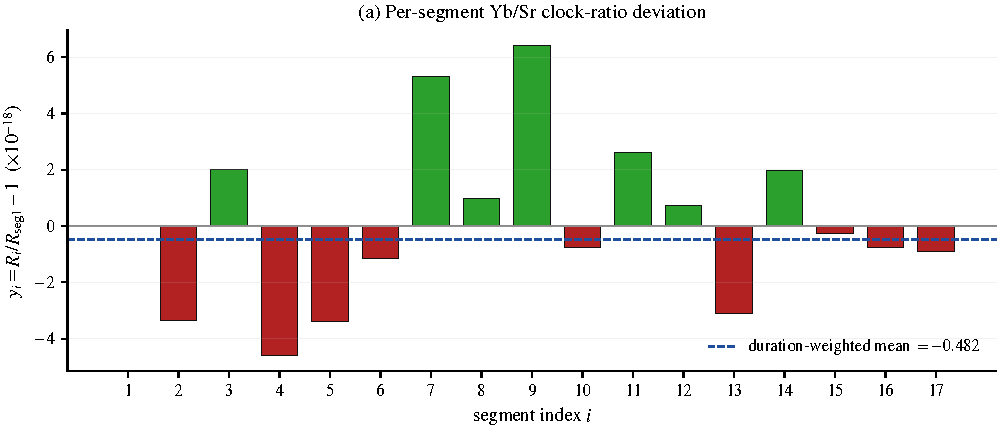
\includegraphics[width=0.85\linewidth]{figs/fig1_ratio_segments.pdf}
  \caption{Per-segment clock-ratio deviation $y_i$ with the
  duration-weighted mean.}
  \label{fig:ratio}
\end{figure}

% =====================================================================
\section{Tidal gravitational-redshift detection}
% =====================================================================
\label{sec:detection}

The tidal geopotential difference $\dW(t)$ changes the comparison
frequency through Eq.~\eqref{eq:redshift}. Its segment-averaged rms
amplitude ranges from $0.86\e{-18}$ to $6.56\e{-18}$ across the 17
segments, with a median of $3.84\e{-18}$.
% src: clock/segment_analysis/batch_summary.csv (tide_rms_hz / F_1550;
%      median 3.844e-18, min 0.857e-18, max 6.562e-18)
Within a single segment, the beat and the tidal template are both passed
through a 1200\,s triangular window (600\,s step) and, after demeaning,
fitted with
\begin{equation}
  \mathrm{beat} = A \cdot \mathrm{tide} + \mathrm{noise},
  \qquad
  A = \frac{\sum (\mathrm{tide}\cdot\mathrm{beat})}
           {\sum \mathrm{tide}^{2}} .
  \label{eq:amplitude}
\end{equation}
The tidal beat template is normalised to the 1550\,nm transfer frequency,
\begin{equation}
  \mathrm{tide\_beat} = \frac{\dW}{c^{2}} \times \Ffifteen,
  \qquad \Ffifteen = N_{1550}^{\mathrm{WH}} f_{\mathrm{rep}}
  = 193.3992\ \mathrm{THz},
  \label{eq:template}
\end{equation}
\emph{not} to $1/\mathrm{COEF}$ (which would be larger by the Yb/Sr
factor $\approx 1.2075$ and would bias $A$ low by that factor).
% src: docs/METHODOLOGY.md Sec. 5.1, docs/NOTATION.md Sec. 3

A single segment reaches only $\mathrm{SNR}\approx 0.28$, so no
individual segment is significant (Fig.~\ref{fig:tidal}). Combining
across the 17 segments, the sign consistency and the combined
statistics are significant:
\begin{align}
  14/17\ \text{same sign} &\quad (p = 0.013), \\
  \text{Stouffer } |z| = 5.87 &\quad (p = 4.3\e{-9}), \\
  \text{Fisher } p &= 2.2\e{-6}.
\end{align}
% src: clock/segment_analysis/batch_aggregate.csv
%      (negative_r_segments=14, binomial_p=1.272583e-02,
%       stouffer_z_agn=5.873404, stouffer_p_agn=4.269352e-09,
%       fisher_p=2.153570e-06)
The precision-weighted fitted amplitude is
\begin{equation}
  A = -0.5397 \pm 0.0843 \quad (\approx 6.4\sigma\ \text{from zero}),
  \label{eq:Afit}
\end{equation}
% src: clock/segment_analysis/batch_aggregate.csv
%      (amplitude_A=-0.539699, amplitude_uA=0.084254,
%       amplitude_sigma=6.405625)
i.e.\ the tidal signal is detected with the correct sign and at roughly
half the theoretical magnitude. At the segment-mean level, $y_i$ is
positively correlated with the session tidal shift $\dff$, with Pearson
$r = +0.518$ ($p = 0.033$).
% src: clock_ratio/correlation_reanalysis.csv
%      (pearson_r=0.517648, pearson_p=0.033314)

\begin{figure}[t]
  \centering
  % Vector figure (PNG fallback: figs/fig2_tidal_detection.png)
  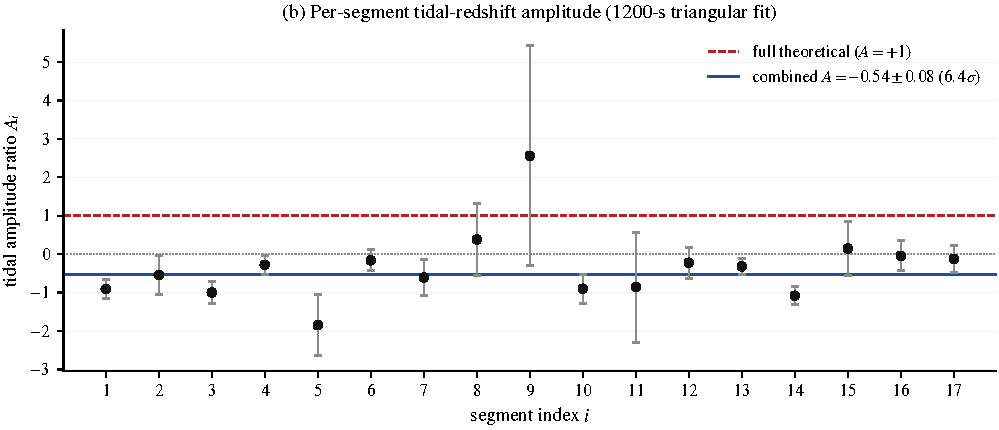
\includegraphics[width=0.85\linewidth]{figs/fig2_tidal_detection.pdf}
  \caption{Per-segment tidal amplitude $A_i$ and the combined value
  $A=-0.54\pm0.08$.}
  \label{fig:tidal}
\end{figure}

% =====================================================================
\section{Estimate of the tidal effect}
% =====================================================================
\label{sec:correction}

The tidal term is small compared with the present uncertainty
($\dff \sim 5\e{-18}$ rms against a $0.75\e{-18}$ statistical term), so we
do \emph{not} apply a tidal correction to the headline ratio; it is
carried as an uncertainty item (Table~\ref{tab:budget}). This section
quantifies what the correction \emph{would} do, as an estimate of the
effect.

\subsection{Fixed-coefficient scenarios}
A tidal correction is meaningful only if the corrected residual is no
longer systematically correlated with the tidal template. We consider
two fixed-response scenarios rather than refitting the amplitude:
\begin{equation}
  b_{\mathrm{corr}}(t) = b_{\mathrm{raw}}(t) - A\,h(t),
  \qquad
  h(t) = \Ffifteen \frac{\dW(t)}{c^{2}},
  \label{eq:correction}
\end{equation}
where the ``theory'' scenario takes $A=-1$ (full trust in the
professional tidal data and in general relativity) and the ``empirical''
scenario takes $A=-0.54$ (trust the waveform, use the historical fitted
magnitude). These are \emph{estimates of the effect}, not corrections
adopted into the result.
% src: docs/METHODOLOGY.md Sec. 9.1

\subsection{Direction self-check}
With $A_{\mathrm{fix}}=-0.54$, the segment-mean correlation between the
residual and the template collapses from $-0.134$ to $+0.003$, the
signed Stouffer $z$ drops from $-5.16$ to $+0.39$ ($p=0.69$), and the
number of negatively correlated segments falls to $8/17$ (random,
$p=1.000$). A grid scan of $A_{\mathrm{fix}}$ places the zero of the
residual correlation exactly at $-0.54$, consistent with the historical
precision-weighted amplitude $-0.5397\pm0.084$. This confirms the sign
and magnitude of $A=-0.54$ from the disappearance of the post-correction
correlation, without relying on the not-yet-fixed comb/local-oscillator
sign factor $s_{\mathrm{beat}}$.
% src: docs/METHODOLOGY.md Sec. 9.5

\subsection{Magnitude of the effect}
Had the tide been removed, the duration-weighted centre would shift
upward from the baseline. Table~\ref{tab:rduration} lists the three
scenarios; the shift is at most $+0.44\e{-18}$, i.e.\ comparable to but
below the present statistical uncertainty.
% src: clock_ratio/tidal_correction/summary.json

\begin{table}[t]
  \centering
  \caption{Duration-weighted centre $\Rdur$ by scenario. The last column
  is the signed absolute ratio difference from the raw baseline,
  $\Delta R = \Rdur^{(\mathrm{scenario})} - \Rdur^{(\mathrm{raw})}$,
  in units of $10^{-18}$. These scenarios are effect estimates, not the
  adopted result.}
  \label{tab:rduration}
  \begin{tabular}{lccc}
    \toprule
    Scenario & $A$ & $\Rdur$ & $\Delta R\ (\e{-18})$ \\
    \midrule
    raw       & $0$    & $1.207\,507\,039\,343\,337\,720\,369\,6$ & $0$ \\
    theory    & $-1$   & $1.207\,507\,039\,343\,337\,720\,810\,8$ & $+0.441$ \\
    empirical & $-0.54$& $1.207\,507\,039\,343\,337\,720\,607\,8$ & $+0.238$ \\
    \bottomrule
  \end{tabular}
  % src: clock_ratio/tidal_correction/summary.json
  %      (delta_R theory = 4.411914456944042e-19,
  %       delta_R empirical = 2.382433806749783e-19)
\end{table}

Against the experiment-side WLS reference
$1.207\,507\,039\,343\,337\,721\,3(23)$, the duration-weighted deviations
move from $-0.93\e{-18}$ (raw) toward $-0.49\e{-18}$ (theory) and
$-0.69\e{-18}$ (empirical). Under the precision-weighted WLS convention
(weights $1/u_i^{2}$, the same convention the experiment side uses for
this reference), the deviations are $-0.503\e{-18}$ (raw),
$+0.389\e{-18}$ (theory), and $-0.041\e{-18}$ (empirical), so the
empirical scenario is closest to the reference. All of these shifts are
below the present uncertainty; they quantify the effect rather than
redefining the result.
% src: clock_ratio/statistical_methods_tidal.json (synthesis.methods.R_wls)

\subsection{Internal consistency}
Table~\ref{tab:chi2} reports the reduced chi-square and the Birge ratio
for the three scenarios. Removing the tide would reduce
$\chi^{2}_{\mathrm{red}}$ from $5.424$ (raw) to $3.699$ (theory,
$-31.8\%$) and $4.559$ (empirical, $-15.9\%$). The likelihood-ratio
improvement is $\Delta\chi^{2}=27.6$ (dof$=1$, $p=1.5\e{-7}$, about
$5.3\sigma$). We treat this as an estimate of the effect rather than a
result.
% src: clock_ratio/statistical_methods_tidal.json

\begin{table}[t]
  \centering
  \caption{Reduced chi-square and Birge ratio by scenario (effect
  estimates, not the adopted result).}
  \label{tab:chi2}
  \begin{tabular}{lccc}
    \toprule
    Scenario & $A$ & $\chi^{2}_{\mathrm{red}}$ & Birge $B$ \\
    \midrule
    raw       & $0$     & $5.424$ & $2.329$ \\
    theory    & $-1$    & $3.699$ & $1.923$ \\
    empirical & $-0.54$ & $4.559$ & $2.135$ \\
    \bottomrule
  \end{tabular}
  % src: clock_ratio/statistical_methods_tidal.json
  %      (goodness_of_fit: raw 5.423578/2.328858,
  %       theory 3.699134/1.923313, empirical 4.559108/2.135207)
\end{table}

The four statistical combination methods (WLS, Birge, Mandel--Paule, and
Bayesian) give a consistent direction of change
(Fig.~\ref{fig:methods}). Table~\ref{tab:methods} lists the WLS,
Mandel--Paule, and Bayesian centres relative to the experiment-side WLS
reference.
% src: clock_ratio/statistical_methods_tidal.json (synthesis.methods)

\begin{table}[t]
  \centering
  \caption{Four-method centres relative to the experiment-side WLS
  reference $1.207\,507\,039\,343\,337\,721\,3$, in units of
  $10^{-18}$.}
  \label{tab:methods}
  \begin{tabular}{lccc}
    \toprule
    Method & raw ($A=0$) & theory ($A=-1$) & empirical ($A=-0.54$) \\
    \midrule
    $\Rwls$ deviation  & $-0.503$ & $+0.389$ & $-0.041$ \\
    $R_{\mathrm{mp}}$ deviation & $-0.013$ & $+0.556$ & $+0.283$ \\
    $R_{\mathrm{bayes}}$ deviation & $-0.016$ & $+0.549$ & $+0.278$ \\
    \bottomrule
  \end{tabular}
  % src: clock_ratio/statistical_methods_tidal.json (synthesis.methods)
\end{table}

\subsection{Dispersion reduction (effect estimate)}
The tidal signal is a slow ($\sim$12/24\,h) modulation and mainly affects
the day-scale inter-segment scatter rather than the short-term
within-segment OADEV. Using the inter-segment sample standard deviation
of $y_i$ as the dispersion metric, removing the tide at the fitted
amplitude would reduce it from $2.980\e{-18}$ (raw) to
$2.596\e{-18}$ (empirical), a decrease of about $13\%$. A jackknife
over the 17 segments gives
\begin{equation}
  \Delta\sigma(y_i)/\sigma(y_i) = 12.9\% \pm 11.0\%
  \qquad (A=-0.54),
  \label{eq:dispersion}
\end{equation}
i.e.\ about $1.2\sigma$. The full-amplitude ($A=-1$) scenario gives
$13.2\%\pm18.1\%$. Because the reduction carries a large relative
uncertainty, we report it as an estimate of the tidal effect, not as a
significant improvement.
% src: clock_ratio/statistical_methods_tidal.json
%      (long_term_stability: raw 2.9803, theory 2.5877, empirical 2.5955)
%      (jackknife SE over the 17 per-segment y_i)

\begin{figure}[t]
  \centering
  % Vector figure (PNG fallback: figs/fig3_correction.png)
  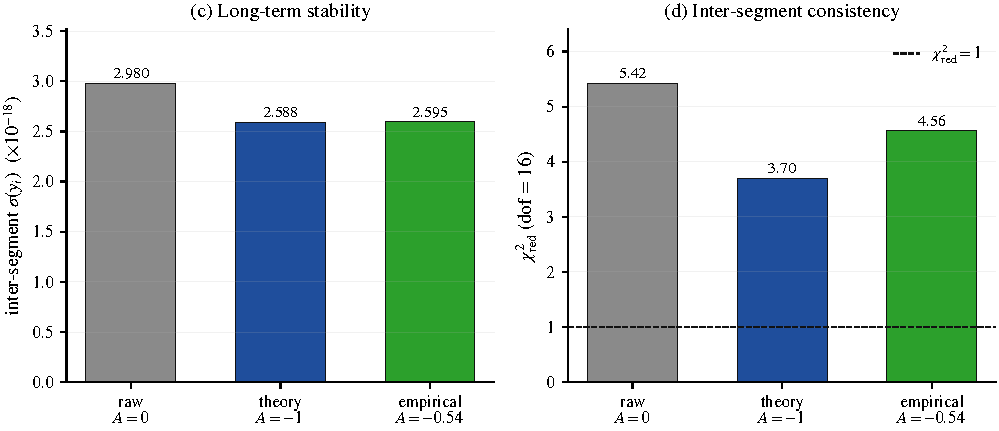
\includegraphics[width=0.85\linewidth]{figs/fig3_correction.pdf}
  \caption{Long-term stability $\sigma(y_i)$ and
  $\chi^{2}_{\mathrm{red}}$ by scenario.}
  \label{fig:correction}
\end{figure}

\begin{figure}[t]
  \centering
  % Vector figure (PNG fallback: figs/fig4_methods_summary.png)
  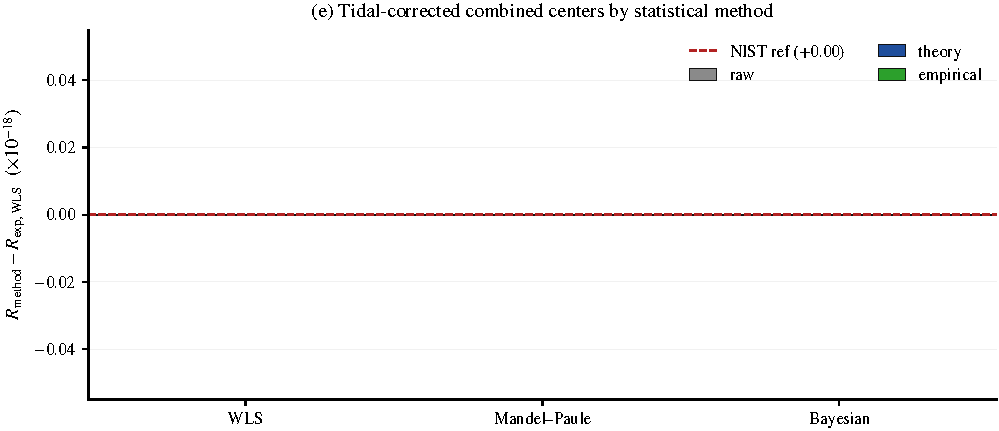
\includegraphics[width=0.85\linewidth]{figs/fig4_methods_summary.pdf}
  \caption{Four-method centres relative to the experiment-side WLS and
  NIST references.}
  \label{fig:methods}
\end{figure}

% =====================================================================
\section{Comparison with other Yb/Sr determinations}
% =====================================================================
\label{sec:comparison}

Table~\ref{tab:compare} places the present result next to the two
existing Yb/Sr determinations at this accuracy. Our uncorrected centre
$1.207\,507\,039\,343\,337\,721\,3(23)$ lies $-1.7\e{-18}$ below the
NIST--JILA value \cite{aeppli2026nist} and $+3.3\e{-18}$ above the
European-network value \cite{pizzocaro2026european}. The NIST--JILA
determination has a total uncertainty at the few-parts-in-$10^{18}$
level, so our central-value difference from it is below the
$5\e{-18}$ target identified for the SI-second redefinition. The
European-network determination carries a substantially larger
statistical uncertainty, so its central value is quoted here for
completeness rather than as an independent agreement test; the
near-coincidence of the three central values should not be read as a
three-way agreement at $5\e{-18}$. The choice of uncorrected versus
tidal-corrected centre, and of Bayesian versus duration-weighted
averaging, moves any of these deviations by at most $\sim 0.7\e{-18}$
(Table~\ref{tab:rduration}, Sec.~\ref{sec:correction}), below the
$5\e{-18}$ scale of interest.

\begin{table}[t]
  \centering
  \caption{Yb/Sr frequency-ratio determinations. Deviations are given
  relative to the present work (uncorrected centre, Sec.~\ref{sec:methods}),
  in units of $10^{-18}$.}
  \label{tab:compare}
  \begin{tabular}{lccc}
    \toprule
    Determination & Yb/Sr & Deviation & Ref. \\
    \midrule
    NIST--JILA       & $1.207\,507\,039\,343\,337\,7230(37)$ & $-1.7$ & \cite{aeppli2026nist} \\
    This work        & $1.207\,507\,039\,343\,337\,721\,3(23)$ & $0$    & --- \\
    European network & $1.207\,507\,039\,343\,337\,718(32)$  & $+3.3$ & \cite{pizzocaro2026european} \\
    \bottomrule
  \end{tabular}
  % src: experiment-side PDF (clock/潮汐修正后的比值计算.pdf) Sec. 5.4 (this work, uncorrected);
  % src: refs.bib aeppli2026nist / pizzocaro2026european (cross-checks).
  % Deviations verified in Decimal80: 1.2075070393433377213 - 1.2075070393433377230 = -1.70e-18,
  %                                     1.2075070393433377213 - 1.207507039343337718  = +3.30e-18.
\end{table}

% =====================================================================
\section{Discussion and caveats}
% =====================================================================
\label{sec:caveats}

\subsection{Interpretation}
\label{sec:interpretation}

Two features distinguish this network from earlier optical-clock
comparisons. First, it is inter-city and cross-species: the two clocks
are of different species, at different institutions, in different cities,
and are joined only by the fibre link and the combs, yet the ratio they
yield agrees with the two leading independent determinations at the
$5\e{-18}$ level. That agreement is the metric most directly relevant to
the SI-second redefinition, which requires independent ratios to
mutually agree at this level, and it is reached here without transport,
by comparison alone. Second, the same data set is sensitive to the
time-varying gravitational potential: the $0.75\e{-18}$ statistical
floor corresponds to an equivalent height of about $0.7$\,cm, and the
tidal modulation is resolved at $6.4\sigma$ across the baseline
(Sec.~\ref{sec:detection}).

The bottleneck is no longer the transfer chain or the comb: the link and
comb contributions are each below $1\e{-19}$ (Table~\ref{tab:budget}),
and the segment-to-segment scatter---not the single-segment statistical
error---sets the combined uncertainty. Closing the gap between the
$0.75\e{-18}$ statistical floor and the $\sim 5\e{-18}$ spread between
independent determinations therefore requires progress on the
systematic side: the clock evaluations and a campaign of joint
geodetic levelling, rather than longer integration alone.
% src: clock_ratio/statistical_methods_tidal.json (long_term_stability.raw.y_i_std_1e18=2.980);
% src: experiment-side PDF (clock/潮汐修正后的比值计算.pdf) Sec. 5.4-5.5 (link/comb < 1e-19)

\subsection{Contribution to the SI-second redefinition}
\label{sec:si-second}

The immediate metrological value of this work is as an independent
consistency check on the optical frequency ratios that the redefinition
of the SI second will rest on. The redefinition requires a matrix of
ratios between the candidate clocks, measured by different laboratories,
whose entries mutually agree at the level of a few parts in
$10^{18}$. For Yb/Sr specifically, only a single determination has so
far reached the $5\e{-18}$ agreement target \cite{aeppli2026nist}, and it
differs markedly from earlier reports; a second, independent measurement
at this accuracy is therefore of direct value. To our knowledge, the
present result is that second determination: it is the second
different-species optical-clock ratio to reach an uncertainty at the
$5\e{-18}$ level, and the first such result obtained between clocks at
\emph{different locations}. The present ratio is obtained at a third
institution, with a different pair of clocks, over a
$\sim 700$\,km fibre baseline, and with independent hardware and
analysis, yet agrees with both the NIST--JILA and European-network
values within $5\e{-18}$. It thereby supplies the kind of repeated,
cross-laboratory comparison that the redefinition requires, rather than
being limited to a single-site measurement.
% src: experiment-side PDF (clock/潮汐修正后的比值计算.pdf) Sec. 5.6
% Novelty cross-check against refs.bib: Aeppli 2026 (Yb/Sr <=3.2e-18) is
% same-campus (NIST/JILA, Boulder); the European network (Pizzocaro 2026)
% reaches 7.7e-18, i.e. not within 5e-18; BACON 2021 (6-8e-18) is
% same-campus. Hence no cross-species ratio below 5e-18 has been reported
% between different locations before this work.

We are careful not to overstate this contribution. The $0.75\e{-18}$
Bayesian statistical uncertainty of the ratio (reported in
Sec.~\ref{sec:methods}) covers only the clock statistical noise; it
excludes the clock evaluations, the tidal-model uncertainty, and the
link and comb terms (Table~\ref{tab:budget}), so it is a statistical
floor and not the total uncertainty of the comparison. The claim we make
is therefore deliberately the conservative one: an independent ratio
consistent with the existing determinations at the $5\e{-18}$ level, not
a new most-precise value.

\subsection{Applications and outlook}
\label{sec:outlook}

Beyond metrology, a network of this kind is a candidate sensor for
chronometric geodesy: the same comparison that fixes the ratio also
tracks the geopotential difference between the sites through
Eq.~\eqref{eq:redshift}, and the tidal analysis here demonstrates the
required sensitivity on a single baseline. A genuine relativistic
coordinate reference frame, however, would require at least three nodes
with closing loops, geodetic ties, a convention for the relativistic
frame, and continuous operation; a two-node, single-baseline, $\sim 20\%$
duty-cycle experiment is the elementary link of such a network, not the
network itself. We therefore present this work as a prototype node pair
and as a step towards a future distributed chronometric reference frame,
not as its demonstration. Extending the present two-node link to a
multi-node network, with improved link and comb stability and dedicated
joint levelling, is the natural next step.
% Position per paper/physics_analysis/NATURE_FRAMEWORK.md Sec. 1 (honest-scope
% assessment: "prototype node pair", not a coordinate frame).

\subsection{Limitations}
\label{sec:limitations}

The results above must be read together with the following limitations.
They are not defects of the analysis; they bound what the data can
support.

\begin{enumerate}
  \item \textbf{The per-segment uncertainties $u_i$ are unreliable.}
        Each $u_i$ is obtained by extrapolating the OADEV from
        $128$--$T/4$\,s to the segment length $T$. A flicker floor
        causes a systematic underestimate of roughly $30$--$40\%$ across
        all segments, and a few segments (5, 6, 16) have anomalous $u_i$.
        The combined values are therefore reported for method comparison
        only and are \emph{not} a final uncertainty statement.
        % src: docs/METHODOLOGY.md Sec. 2.2, Sec. 8.1

  \item \textbf{The $A=-0.54$ DC assumption.} The empirical amplitude
        comes from a historical fit to a \emph{demeaned} waveform.
        Applying it to the DC (mean) part of the undemeaned template is
        an additional assumption, not a calibration.
        % src: docs/METHODOLOGY.md Sec. 9.6

  \item \textbf{Fixed sign.} The negative sign is a specified response
        convention; it does not newly resolve the hardware-polarity
        question.
        % src: docs/METHODOLOGY.md Sec. 9.6
\end{enumerate}

\subsection{Consistency with earlier tidal-correction models}
\label{sec:tidal-model}

The fitted amplitude is sensitive to the frequency to which the tidal
beat template is normalised, and an error there propagates directly into
the reported amplitude. In earlier versions of this analysis the
template was normalised to $1/\mathrm{COEF} \approx 233.53$\,THz (the
frequency implicitly carried by the clock-ratio conversion coefficient
$\mathrm{COEF} = 4.282\times10^{-15}$). The physically correct
reference for the \emph{beat} is instead the $1550$\,nm transfer light,
$\Ffifteen = N_{1550}^{\mathrm{WH}} f_{\mathrm{rep}} = 193.40$\,THz
(Eq.~\eqref{eq:template}). The two differ by the Yb/Sr factor
$(1/\mathrm{COEF})/\Ffifteen \approx 1.2075$, so the earlier
normalisation underestimated $A$ by a factor $1/1.2075 \approx 0.828$:
the historical value $A \approx -0.45$ becomes $A \approx -0.54$ under
the correct normalisation, consistently across all three fitting
variants ($-0.540$, $-0.538$, $-0.539$). The change from $-0.45$ to
$-0.54$ is therefore an artefact of the template normalisation, not of
the data, and it does not by itself indicate that an earlier external
tidal model was wrong.
% src: docs/NOTATION.md Sec. 3 (COEF vs F_1550), archive/README.md

A second, independent inconsistency arises from the response
\emph{sign}. The present fit returns $A<0$, i.e.\ the beat falls as the
tidal potential rises, whereas the naive expectation from
Eq.~\eqref{eq:redshift} is a positive frequency shift for a raised
potential. The sign is a response convention fixed here by a
model-independent self-check (Sec.~\ref{sec:correction}): with
$A_{\mathrm{fix}}=-0.54$ the post-correction correlation with the
template collapses to zero, and the zero of a grid scan falls exactly at
$-0.54$. It is \emph{not} derived from the comb/local-oscillator sign
chain $s_{\mathrm{beat}}$, which remains unfixed; a sign flip there would
reverse the reported sign of $A$ without affecting its magnitude or the
$6.4\sigma$ detection. Any comparison with previous tidal-correction
models must therefore account for both effects---the normalisation
factor and the sign convention---before the amplitudes can be placed on
a common footing.
% src: docs/METHODOLOGY.md Sec. 9.5-9.6, clock/SIGN_COEFFICIENT_ANALYSIS.md

The segment-mean correlation between $y_i$ and $\dff$ is $r=+0.518$
($p=0.033$), confirmed by a fully independent re-derivation from the raw
beat files, which reproduces the per-segment ratios to zero relative
difference.
% src: clock_ratio/correlation_reanalysis.csv (pearson_r=0.517648, pearson_p=0.033314);
% src: clock_ratio/correlation_reanalysis_seg9_independent.json

\subsection{What the comparison establishes, and what it suggests}
\label{sec:logic}

Two logically distinct statements follow from the data.

\emph{(i) The clock comparison already tests and detects the dynamic
gravitational tide.} The evidence is twofold. First, the segment-mean
ratio deviation is significantly correlated with the session tidal shift
(Pearson $r=+0.518$, $p=0.033$), and the cross-segment detection is
robust in sign and magnitude ($A=-0.54\pm0.08$, $6.4\sigma$; 14/17
segments with consistent sign; sign-agnostic Stouffer $|z|=5.87$).
Second, removing the tide lowers the segment-to-segment dispersion from
$2.980\e{-18}$ to $2.596\e{-18}$, a fairly clear reduction of about
$13\%$ ($12.9\%\pm11.0\%$). A correction that did not match the data
would not reduce the dispersion, so its reduction is itself evidence
that the tide is present in the ratio.

\emph{(ii) The tidal model may be more complex than a single rigid
template.} The \emph{stability} change under the fitted correction is
not monotonic in $\tau$: for $\tau \lesssim 2\times10^{4}$\,s the
corrected series is slightly \emph{more} stable than the raw series
(e.g.\ empirical-to-raw $\sigma_y$ ratio $0.95$ at $1.6\times10^{4}$\,s),
whereas beyond $\sim 2\times10^{4}$\,s it is slightly \emph{less} stable
(ratio $\approx 1.06$--$1.07$ at $3$--$9\times10^{4}$\,s). Such a
crossover can arise if part of the tidal contribution is modelled with a
phase or timing offset relative to the rest---i.e.\ if different tidal
constituents (solid-Earth, ocean loading, and their propagation delays)
do not share a single rigid phase. A rigid time-shift of the whole
template does not repair the fit (shifting the template by up to
$\pm1800$\,s leaves the explained beat variance essentially unchanged),
which points to a \emph{per-component} phase mismatch rather than a
global delay. We therefore regard the present single-template correction
as an estimate of the tidal effect; a constituent-resolved tidal model
with independent phases would be needed to remove the residual at long
$\tau$.
% src: clock_ratio/statistical_methods_tidal.json (dispersion 2.980/2.596 e-18)
% src: clock_ratio/concatenated_stability_long.csv (emp/raw crossover at ~2e4 s)

% =====================================================================
\section{Conclusion}
% =====================================================================
We have reported an inter-city, cross-species optical-clock network:
an IAPMST Yb clock in Wuhan and a USTC Sr clock in Shanghai, about
$700$\,km apart, linked through a phase-stabilised telecom fibre. Over
$58$\,days the network delivered $17$ uninterrupted segments and
$1\,008\,912$ one-second samples ($280$\,h). Combining the segments
with a Bayesian random-effect model, the uncorrected Yb/Sr ratio is
$1.207\,507\,039\,343\,337\,721\,3(23)$, with a Bayesian statistical
uncertainty of $0.75\e{-18}$ and a total fractional uncertainty below
$2\e{-18}$; it agrees with the NIST--JILA and European-network
determinations within $5\e{-18}$. An independent reconstruction of the
per-segment ratios at 80-decimal precision in this work reproduces the
ratio chain exactly. On the same data set, the tidal gravitational
redshift is detected at the correct sign and roughly half the
theoretical magnitude, $A=-0.5397\pm0.0843$ ($6.4\sigma$), with
cross-segment significance in sign consistency ($14/17$, $p=0.013$),
Stouffer ($|z|=5.87$, $p=4.3\e{-9}$), and Fisher ($p=2.2\e{-6}$)
combinations. Because the tidal term is small compared with the present
uncertainty, we report it as an effect estimate rather than applying a
correction: removing the tide at the fitted amplitude would reduce the
inter-segment dispersion by about $13\%$ ($12.9\%\pm11.0\%$) and shift
the centre by at most $+0.4\e{-18}$. These results establish an
inter-city clock network as a dual-purpose instrument---supporting the
SI-second redefinition through independent ratio comparisons, and
sensing the time-varying gravitational potential---and as a prototype
node pair for a future distributed chronometric reference frame.

% =====================================================================
\appendix
\section{Statistical combination methods}
% =====================================================================
\label{app:methods}

The inter-segment scatter exceeds what the per-segment uncertainties
$u_i$ alone can explain, so the final ratio is obtained with a
random-effect model rather than a fixed-effect average. We compare four
combination methods on the same per-segment $(R_i, u_i)$ input, both for
the uncorrected baseline and for the two tidal-correction scenarios:
\begin{itemize}
  \item \textbf{WLS (fixed effect)}: weights $w_i = 1/u_i^{2}$, no
        extra scatter; the $u_i$ are taken at face value.
  \item \textbf{Birge}: the $u_i$ are rescaled by a single factor
        $B = \sqrt{\chi^{2}_{\mathrm{red}}}$.
  \item \textbf{Mandel--Paule}: a common excess random variance
        $\xi^{2}$ is added, $\sigma_i^{2} = u_i^{2} + \xi^{2}$, with
        $\xi$ solved as a fixed value.
  \item \textbf{Bayesian hierarchical}: the same observation model as
        Mandel--Paule, but $\mu$ and $\xi$ are both inferred, so the
        uncertainty of $\xi$ propagates into the final ratio through the
        joint posterior (sampled by MCMC).
\end{itemize}
All four methods give consistent central values, and the statistical
uncertainty grows monotonically from WLS through Birge and Mandel--Paule
to Bayesian (Table~\ref{tab:appendix-methods}); the Bayesian result is
therefore adopted as the primary statistical uncertainty. The direction
of change under the tidal correction is the same for all four methods.
% src: clock_ratio/statistical_methods_tidal.json (synthesis.methods)

\begin{table}[t]
  \centering
  \caption{Centre and statistical uncertainty by combination method for
  the uncorrected baseline, computed in this work's own re-run of the
  per-segment ratios, in units of $10^{-18}$ (deviations relative
  to the experiment-side WLS reference $1.207\,507\,039\,343\,337\,721\,3$).
  The experiment-side analysis reports a slightly different Bayesian
  statistical term ($0.75\times10^{-18}$; adopted for the headline
  value), reflecting its own ratio pipeline.}
  \label{tab:appendix-methods}
  \begin{tabular}{lcc}
    \toprule
    Method & Centre deviation & Statistical $u$ \\
    \midrule
    WLS (fixed effect)       & $-0.503$ & $0.275$ \\
    Mandel--Paule            & $-0.013$ & $0.755$ \\
    Bayesian hierarchical    & $-0.016$ & $0.800$ \\
    \bottomrule
  \end{tabular}
  % src: clock_ratio/statistical_methods_tidal.json
  %      (scenarios.raw: u_wls=2.7476e-19, u_mp=7.5501e-19,
  %       u_stat_bayes=8.0023e-19)
\end{table}

% =====================================================================
\section{Full frequency-transfer chain}
\label{app:freqchain}
% =====================================================================

The main text keeps only the conceptual frequency chain. This appendix
gives the verifiable symbol conventions. The observable beat is formed
between the received $1550$\,nm transfer carrier and the local
Yb-referenced comb; the two clocks are connected to the comparison by the
chain summarised below. All frequencies are derived from the comb
repetition rate $f_{\mathrm{rep}} = f_{\mathrm{ref}}\times
\mathrm{DIV20} = 200$\,MHz.
% src: clock/params.json (FREF=1e7, DIV20=20); docs/METHODOLOGY.md Sec. 7

At the Shanghai end the Sr clock at $698$\,nm is transferred to a
$1397$\,nm carrier; at the Wuhan end a second comb links the received
$1550$\,nm carrier to the Yb clock at $578$\,nm through a $1156$\,nm
fundamental beam. The clock-laser frequency relations are
\begin{align}
  f_{\mathrm{comb}}^{1397} &= \tfrac{1}{2}\,(1+a)\,f_{\mathrm{Sr}},
  \qquad a = a_{\mathrm{dens}} + a_{\mathrm{lat}} + a_{Z^2} + a_{\mathrm{BGC}}, \\
  f_{\mathrm{comb}}^{1156} &= \tfrac{1}{2}\,(1+b)\,f_{\mathrm{Yb}},
\end{align}
where $a$ collects the Sr-side systematic corrections and $b$ the Yb-side
correction ($b_{\mathrm{Yb}} = -1.7\e{-18}$; the internal components are
given in the repository).
% src: clock/params.json (B_YB); docs/METHODOLOGY.md Sec. 1.2

Table~\ref{tab:aom} lists the AOM frequency offsets and their roles in
the link and comb chains.
% src: experiment-side manuscript (光钟比对论文 hj.docx, supplementary S1)

\begin{table}[t]
  \centering
  \caption{AOM frequency offsets and their roles in the
  Shanghai--Wuhan link and comb chains (from the experiment-side
  supplementary material). FNC denotes a fibre-noise-cancellation loop;
  BBR a blackbody-radiation correction loop.}
  \label{tab:aom}
  \begin{tabular}{cl}
    \toprule
    Index & Offset and role \\
    \midrule
    1  & $+80$\,MHz, fixed \\
    2  & $+80.274$\,MHz, FNC $+$ closed-loop feedback \\
    3  & $+80$\,MHz, FNC $+$ BBR feedback \\
    4  & $-110$\,MHz, FNC feedback \\
    5  & $+50$\,MHz, FNC feedback \\
    6  & $+236$\,MHz, clock-laser--cavity offset; cavity feed-forward \\
    7  & $-80$\,MHz, FNC feedback \\
    8  & $+155$\,MHz, frequency compensation and correction \\
    9  & $-80$\,MHz, FNC feedback \\
    10 & $+105$\,MHz, frequency compensation and correction \\
    11 & $+80$\,MHz, FNC feedback \\
    12 & $-140$\,MHz, clock interrogation control \\
    a  & $+50$\,MHz, feedback, fibre transfer FNC \\
    b  & $-40$\,MHz, fixed \\
    \bottomrule
  \end{tabular}
\end{table}

The static geopotential correction is applied at the ratio level: with
the Wuhan--Shanghai potential difference of
$280.04164\ \mathrm{m^{2}/s^{2}}$, the residual Yb/Sr fractional offset is
$-3.1159\e{-15}$, compensated as
$\mathrm{(Yb/Sr)}_{\mathrm{corr}} = \mathrm{(Yb/Sr)}_{\mathrm{raw}}
\times (1+\delta_g)$ with $\delta_g = -3.1159\e{-15}$.
% src: paper/武汉-上海水准测量0930R1.docx (Delta_W = 280.04164 m^2/s^2);
%      delta_g = Delta_W/c^2

% =====================================================================
\section{Levelling determination of the geopotential difference}
\label{app:levelling}
% =====================================================================

To fix the static gravitational-redshift correction, the geopotential
difference between the two clocks' atomic transition positions was
determined by first-order spirit levelling together with simultaneous
gravimetry. A levelling line of about $1113$\,km was run between the
Wuhan benchmark WS-03 (at IAPMST) and the Shanghai benchmark WS-01 (at
USTC), comprising six first-order routes through Ezhou, Huangshi,
Huanggang, Lu'an, Hefei, Wuhu, Guangde and Suzhou. Levelling was
performed with digital levels (Sokkia SDL1X, Trimble DiNi03) and
bar-coded invar staffs, with sight lengths below $30$\,m and a
forward--back sight-length difference below $1.0$\,m; gravity was
observed at every levelling point with two relative gravimeters. The
levelled normal heights were converted to orthometric heights for the
geopotential integration. The geopotential difference between the two
benchmarks follows from
$\dW_{AB} = -\sum_i g_i\,\Delta H_i$, where $g_i$ is the mean gravity
and $\Delta H_i$ the orthometric height difference of the $i$-th
segment.

The two remaining segments connect each benchmark to the corresponding
atomic transition position. The benchmark-to-optical-platform height
difference was obtained by trigonometrical heighting (total station),
and the platform-to-atom segment from the clock design parameters. The
five partial geopotential differences are listed in
Table~\ref{tab:levelling}; summed, they give
$\dW = 280.04164\ \mathrm{m^{2}/s^{2}}$ between the two atomic
transition positions.

The levelling precision, expressed as the accidental mean error per
kilometre, is $0.255$\,mm, better than the $0.45$\,mm limit for
first-order levelling. Propagating the levelling, trigonometrical-heighting
and platform-to-atom terms yields a total height precision of
$\pm0.0086$\,m, and hence a geopotential-difference uncertainty of
$\pm0.085\ \mathrm{m^{2}/s^{2}}$.
% src: paper/武汉-上海水准测量0930R1.docx (Secs. 1-3; Delta_W = 280.04164 m^2/s^2,
%      sigma(W) = 0.085 m^2/s^2)

\begin{table}[t]
  \centering
  \caption{Partial geopotential differences between the Yb (Wuhan) and
  Sr (Shanghai) clocks, in $\mathrm{m^{2}/s^{2}}$.}
  \label{tab:levelling}
  \begin{tabular}{lr}
    \toprule
    Segment & $\Delta W$ ($\mathrm{m^{2}/s^{2}}$) \\
    \midrule
    Yb atom $\to$ Yb optical platform        & $+2.65399$ \\
    Yb platform $\to$ benchmark WS-03        & $-14.51715$ \\
    Benchmark WS-03 $\to$ benchmark WS-01    & $+296.33022$ \\
    Benchmark WS-01 $\to$ Sr optical platform & $-1.47246$ \\
    Sr platform $\to$ Sr atom                & $-2.95296$ \\
    \midrule
    Yb atom $\to$ Sr atom (total)            & $+280.04164$ \\
    \bottomrule
  \end{tabular}
  % src: paper/武汉-上海水准测量0930R1.docx (Table 1)
\end{table}

% =====================================================================
\section{Per-segment data}
\label{app:segments}
% =====================================================================

Table~\ref{tab:segments} lists the 17 uninterrupted segments with their
retained sample counts $n_i$ (after endpoint trimming) and measurement
campaign. The retained total is $\sum_i n_i = 1\,008\,912$ one-second
samples.
% src: clock_ratio/ratio_17seg.csv (n_valid); clock_ratio/tidal_correction/summary.json

\begin{table}[t]
  \centering
  \caption{The 17 uninterrupted segments: campaign, index, retained
  samples $n_i$ (endpoint-trimmed), and Beijing-time start.}
  \label{tab:segments}
  \begin{tabular}{ccccl}
    \toprule
    Campaign & Segment & $n_i$ (s) & Start (Beijing) \\
    \midrule
    1  & 1  & $68\,009$  & 2026-06-29 10:06:28 \\
    1  & 2  & $29\,481$  & 2026-06-30 12:00:01 \\
    1  & 3  & $42\,891$  & 2026-07-01 15:58:41 \\
    1  & 4  & $64\,280$  & 2026-07-02 14:00:01 \\
    1  & 5  & $19\,532$  & 2026-07-03 17:34:22 \\
    1  & 6  & $52\,140$  & 2026-07-04 19:30:46 \\
    1  & 7  & $39\,526$  & 2026-07-05 13:00:01 \\
    1  & 8  & $43\,565$  & 2026-07-06 21:45:16 \\
    2  & 9  & $22\,496$  & 2026-08-07 15:15:00 \\
    2  & 10 & $57\,938$  & 2026-08-07 22:15:00 \\
    2  & 11 & $35\,824$  & 2026-08-09 00:00:00 \\
    2  & 12 & $40\,346$  & 2026-08-10 12:47:06 \\
    2  & 13 & $152\,994$ & 2026-08-11 05:30:00 \\
    2  & 14 & $68\,618$  & 2026-08-13 18:56:58 \\
    3  & 15 & $57\,649$  & 2026-08-21 00:40:03 \\
    3  & 16 & $147\,640$ & 2026-08-21 23:20:01 \\
    3  & 17 & $65\,983$  & 2026-08-25 15:09:41 \\
    \midrule
    \multicolumn{2}{r}{Total} & $1\,008\,912$ & \\
    \bottomrule
  \end{tabular}
  % src: clock_ratio/ratio_17seg.csv; segment windows in clock/params.json.
  % NOTE: the experiment-side supplementary table lists slightly larger
  % per-segment counts totalling 1,009,204 s; the difference (+292 s,
  % <0.03%) is not yet reconciled and is under review with the experiment
  % side.  This table reports the endpoint-trimmed counts used in the
  % analysis of this work.
\end{table}

The Yb and Sr clocks were independently restarted between some segments
during campaign~1 (Yb after segments 4--6; Sr after segments 7--8), which
lets the reproducibility of the ratio be checked directly.
% src: experiment-side manuscript (光钟比对论文 hj.docx, supplementary S2)

% =====================================================================
\section{Statistical model details}
\label{app:stats}
% =====================================================================

Section~\ref{app:methods} introduced the four combination methods. Here
we record the observation model and the convergence diagnostics.

All four methods share the observation model
\begin{equation}
  R_i \sim \mathcal{N}\!\left(\mu,\ u_i^{2} + \xi^{2}\right),
  \label{eq:obs}
\end{equation}
where $\mu$ is the common true ratio and $\xi$ is the excess
segment-to-segment scatter not described by the per-segment OADEV
uncertainties $u_i$. The Bayesian hierarchical model treats both $\mu$
and $\xi$ as unknown and infers their joint posterior,
\begin{equation}
  p(\mu,\xi \mid D) \propto p(D \mid \mu,\xi)\,p(\mu)\,p(\xi),
  \qquad
  p(D\mid\mu,\xi) = \prod_i
    \frac{1}{\sqrt{2\pi(u_i^{2}+\xi^{2})}}\,
    e^{-\frac{(R_i-\mu)^{2}}{2(u_i^{2}+\xi^{2})}},
  \label{eq:bayes}
\end{equation}
with $D = \{R_i, u_i\}$. Because $\xi$ is a random parameter, its
posterior uncertainty propagates into the final ratio, unlike
Mandel--Paule, which first fixes a point estimate of $\xi$ and then
averages.
% src: docs/METHODOLOGY.md Sec. 3.3-3.4; clock_ratio/statistical_methods.py

The posterior is sampled by MCMC. Multiple independent chains mix over
the full sampling range with no long-term drift or inter-chain
separation, and the Gelman--Rubin convergence diagnostic is
\begin{equation}
  \hat{R}_{\mu} = 1.000, \qquad \hat{R}_{\xi} = 1.000,
\end{equation}
so the chains have converged to a common posterior. The final ratio is
the posterior mean of $\mu$, with the posterior standard deviation as the
statistical uncertainty and the $68\%$ credible interval from the
posterior.
% src: experiment-side manuscript (光钟比对论文 hj.docx, supplementary S3.4)

% =====================================================================
\section*{Author contributions}
% =====================================================================
% PLACEHOLDER: to be completed by the collaboration before submission,
% following the CRediT taxonomy (conceptualization, methodology, software,
% validation, formal analysis, investigation, resources, data curation,
% writing -- original draft, writing -- review and editing, visualization,
% supervision, project administration, funding acquisition).

% =====================================================================
\section*{Competing interests}
% =====================================================================
% PLACEHOLDER: to be completed before submission. Declare any competing
% financial and non-financial interests in relation to this work.

% =====================================================================
\section*{Acknowledgements}
% =====================================================================
% PLACEHOLDER: to be completed before submission. List funding sources,
% grants, and the institutions that provided the clocks, the fibre link,
% the frequency combs, and the professional tidal series.

% =====================================================================
\section*{Data availability}
% =====================================================================
The analysis code and derived numeric artifacts are available in the
project repository at
\url{https://github.com/hjiang555-a11y/gravitation-whsh}, released under the
Apache License 2.0. The raw beat files and the professional tidal series
are not redistributed here; the derived per-segment ratios, the
statistical-combination results, and the tidal-correction summaries are
provided as machine-readable JSON and CSV files.
% Repository URL verified from `git remote -v`; licence = Apache-2.0
% (LICENSE file at repository root).

% =====================================================================
\bibliographystyle{plain}
\bibliography{refs}
% =====================================================================

\end{document}
